\chapter{Πολυκατηγορική Ταξινόμηση με τον GMl-ASLCS$_{\:0}$}
\label{gmlaslcs0}
Η παρούσα εργασία ερείδεται επί της Διπλωματικής Εργασίας του Μίλτου Αλλαμανή \cite{allamanis11} και του Μανθάνοντος Συστήματος Ταξινομητών που ανέπτυξε. Το ΜαΣΤ αυτό θα το ονομάσουμε, στα πλαίσια αυτής της εργασίας, GMl-ASLCS$_{\:0}$. Η ονομασία, εκ πρώτης όψης, προσομοιάζει στο ΜαΣΤ που αναφέραμε στο προηγούμενο κεφάλαιο, τον AS-LCS. Στην πραγματικότητα, είναι η επέκτασή του, η προσαρμογή του, στον πολυκατηγορικό ($Ml$) χώρο, όπως ακριβώς και οι αλγόριθμοι που παρουσιάσαμε στην Παρ. (\ref{subsec:algorithmAdjustment}). Ο GMl-ASLCS$_{\:0}$ κληρονομεί τις  βασικές λειτουργίες του πλαισίου λειτουργίας του AS-LCS, όπως τις παραμέτρους των κανόνων που εξελίσσει, και επεκτείνει άλλες, στο πολυκατηγορικό πεδίο. Η μηδενική υποσημείωση στην ονομασία του GMl-ASLCS$_{\:0}$ γίνεται για να καταδείξουμε ότι αυτό το σύστημα είναι η αφετηρία από όπου ξεκινάμε τη μελέτη, την ανάλυσή και την επέκτασή μας. Ο GMl-ASLCS$_{\:0}$ είναι μία από τις πρώτες προσεγγίσεις του προβλήματος της πολυκατηγορικής (ή πολυετικετικής) ταξινόμησης με μεθόδους Εξελικτικής Υπολογιστικής. Η μελέτη του στα πλάισια των \cite{allamanis11} και \cite{DBLP:conf/icannga/allamanis13} παρέχει τις πρώτες ενδείξεις πως η πολυκατηγορική ταξινόμηση με ΜαΣΤ είναι εφικτή, ενώ υπάρχει χώρος για βελτίωση, ώστε ο GMl-ASLCS$_{\:0}$ να μπορέσει να ανταγωνιστεί αποτελεσματικότερα τους state-of-art αλγορίθμους στο χώρο της πολυκατηγορικής ταξινόμησης.


Σε αυτό το κεφάλαιο: 

\begin{itemize}
\item παρουσιάζουμε τις αλλαγές που ήταν απαραίτητο να γίνουν στον AS-LCS ώστε να είναι σε θέση να ταξινομεί πολυκατηγορικά δείγματα, παρέχοντας έτσι το υπόβαθρο για την κατανόηση του GML-ASLCS$_{\:0}$ και του μοντέλου που αναπτύξαμε,
\item επισκεπτόμαστε, παράλληλα, τις βασικές συνιστώσες του GML-ASLCS$_{\:0}$, και
\item μπαίνουμε σε μεγαλύτερο βάθος σε ορισμένες λειτουργίες του, ώστε να γίνουν κατανοητοί οι λόγοι για τους οποίους τις τροποποιούμε.
\end{itemize}

\section{Τροποποίηση της Αναπαράστασης Κανόνων}
Η Αναπαράσταση των Κανόνων που χρησιμοποιούνται από ένα ΜαΣΤ μονοκατηγορικής ταξινόμησης τροποποιείται, ώστε στο τμήμα συνθήκης των κανόνων να περιλαμβάνεται η απόφαση για πολλαπλές ετικέτες. Προτού αναφερθούμε στην αναπαράσταση των ετικετών, εξετάζουμε την αναπαράσταση του τμήματος συνθήκης για τους διαφορετικούς τύπους γνωρισμάτων: τα \emph{δυαδικά}, \emph{ονομαστικά} και \emph{πραγματικά} γνωρίσματα.

\subsection{Αναπαράσταση Δυαδικών Γνωρισμάτων}
Οι διαθέσιμες τιμές για ένα δυαδικό γνώρισμα είναι τρεις: \emph{Αληθής}, \emph{Ψευδής}, και \emph{Αδιαφορία} (\#). Ο χαρακτήρας \# συμβολίζει την αδιαφορία ενός κανόνα για την τιμή του αντίστοιχου γνωρίσματος στα δεδομένα εισόδου. Συνεπώς, ένας κανόνας της μορφής $111\# \Rightarrow 101$ καλύπτει \emph{τουλάχιστον δύο} δείγματα: το $1111 \Rightarrow 101$, και το $1110 \Rightarrow 001$. Λόγω της ύπαρξης τριών πιθανών καταστάσεων για την τιμή ενός δυαδικού γνωρίσματος, χρησιμοποιούνται δύο δυαδικά ψηφία για την αναπαράστασή της. Ένα δυφίο, το λεγόμενο \emph{Ψηφίο Ενεργοποίησης}, καθιστά το \emph{Ψηφίο Τιμής} σχετικό ή άσχετο: εάν το Ψηφίο Ενεργοποίησης έχει τιμή μηδέν, ο κανόνας που το περιέχει αδιαφορεί για το συγκεκριμένο γνώρισμα. Σε αντίθετη περίπτωση, η τιμή του γνωρίσματος ταυτίζεται με την τιμή  του Ψηφίου Τιμής.

$$ \overbrace{
\underbrace{b_{1}}_\text{ψηφίο ενεργοποίησης} \:
\underbrace{b_{0}}_\text{ψηφίο τιμής}}
^\text{Συνθήκη Δυαδικού Γνωρίσματος}$$

\subsection{Αναπαράσταση Ονομαστικών Γνωρισμάτων}
Η αναπαράσταση ονομαστικών γνωρισμάτων αποτελεί γενίκευση αυτής των δυαδικών. Περιέχει και αυτή ένα ψηφίο ενεργοποίησης και, για την αναπαράσταση των $n$ τιμών ενός ονομαστικού γνωρίσματος, χρησιμοποιεί μία δυαδική μάσκα $n$ δυφίων. Μία μη μηδενική τιμή ενός από αυτά τα δυφία υποδηλώνει την αντίστοιχη τιμή του ονομαστικού γνωρίσματος. Όταν η μάσκα ενεργοποίησης τιμών εφαρμοσθεί σε ένα δείγμα και προκύψει τιμή διάφορη του μηδενός, τότε το δείγμα ικανοποιεί τη συγκεκριμένη συνθήκη του κανόνα.

$$ \overbrace{
\underbrace{b_{n}}_\text{Ψηφίο Ενεργοποίησης}
\underbrace{b_{n-1}b_{n-2}
\dots b_{1}b_{0}}_\text{μάσκα τιμών}
}^\text{Συνθήκη Ονομαστικού Γνωρίσματος}$$

\subsection{Αναπαράσταση Συνθηκών Πραγματικών Γνωρισμάτων}
Για την αναπαράσταση συνθηκών πραγματικών γνωρισμάτων επιλέχθηκε η αναπαράσταση \emph{διαστήματος τιμών}, η οποία ορίζει ένα διάστημα επιτρεπτών τιμών για το γνώρισμα στο οποίο αναφέρεται, καθιστώντας εφικτή και τη δημιουργία μονόπλευρων ανισοτήτων. Επιπρόσθετα, επιλέχτηκε η αναπαράσταση θέσης για την κωδικοποίηση των εμπλεκομένων πραγματικών αριθμών. Στην αναπαράσταση θέσης, επειδή η μέγιστη και η ελάχιστη τιμή ενός γνωρίσματος είναι εκ των προτέρων γνωστές, κβαντίζονται οι ενδιάμεσες τιμές και αντιστοιχίζονται στις προκύπτουσες στάθμες τα δυαδικά ψηφία που χρησιμοποιούνται για την αναπαράσταση ενός αριθμού. Με αυτόν τον τρόπο, χρησιμοποιούνται, μεν, όλα τα διαθέσιμα δυαδικά ψηφία χωρίς να υπάρχει η ανάγκη για διόρθωση, καθίσταται δε πολυπλοκότερος ο υπολογισμός του πραγματικού αριθμού στον οποίο αντιστοιχεί το γονίδιο. Πιο συγκεκριμένα:
\\

\begin{equation} 
x_{i}=min_{i}+\frac{int(gene_{i})}{2^b}(max_{i} - min_{i}) 
\end{equation}  
\\
όπου $x_{i}$ η πραγματική τιμή του γνωρίσματος $i$, $max_{i}$ και $min_{i}$ η καθολική μέγιστη και ελάχιστη τιμή του γνωρίσματος αντίστοιχα, $b$ ο αριθμός των δυαδικών ψηφίων που χρησιμοποιήθηκαν στην αναπαράσταση και $gene_{i}$ η δυαδική αναπαράσταση του γονιδίου. Να σημειωθεί ότι το $b$ είναι μια παράμετρος με την οποία μπορεί να ελεγχθεί η διακριτική ικανότητα του κανόνα. Μεγαλύτερες τιμές του $b$, οδηγούν σε μεγαλύτερη ακρίβεια, με κόστος την αύξηση του μεγέθους του γονιδίου. Συνολικά, με βάση την αναπαράσταση των πραγματικών τιμών που επιλέχθηκε, για $2^{k}$ στάθμες κβαντισμού, η δομή των συνθηκών πραγματικών γνωρισμάτων μπορεί να αποδοθεί σχηματικά ως εξής:
\\

$$ \overbrace{
\underbrace{b_{2k}}_\text{ψηφίο ενεργοποίησης}
\underbrace{b_{2k-1}b_{2k-2}
\dots b_{k+1}b_{k}}_\text{άνω όριο}
\underbrace{b_{k-1}b_{k-2
}\dots b_1b_0}_\text{κάτω όριο}}
^\text{Συνθήκη Πραγμ. Γνωρισμάτων με Αναπαράσταση Διαστήματος Τιμών}$$
\\

\subsection{Αναπαράσταση του Τμήματος Απόφασης}
Η αναπαράσταση των κατηγοριών - ετικετών είναι σαφέστατα κρίσιμης σημασίας. Στην κατηγοριοποίηση μίας κατηγορίας, η αναπαράσταση είναι κάτι το τετριμμένο: οι πιθανές τιμές της μοναδικής ετικέτας - απόφασης αναπαριστώνται ως φυσικοί αριθμοί και ενσωματώνονται στην αναπαράσταση του γονιδίου ως δυαδικοί. Στην πολυκατηγορική ταξινόμηση υπάρχει μεγάλος χώρος για εναλλακτικές προσεγγίσεις - από την \emph{αναπαράσταση μόνο μίας ετικέτας}, όπως στην απλή κατηγοριοποίηση, μέχρι τη \emph{σαφή αναπαράσταση όλων των ετικετών} και την \emph{αναπαράσταση ετικετών με αδιαφορίες}. Στον GMl-ASLCS$_{\:0}$ επιλέχθηκε η τελευταία, καθώς η πρώτη προσεγγίζει τη μέθοδο μετασχηματισμού προβλημάτων $BR$, ή αν αναπαρασταθούν όλες οι ετικέτες στο ίδιο ΜαΣΤ, τη μέθοδο $RT$. Η δεύτερη προσέγγιση, από την άλλη, έχει ως αποτέλεσμα την παραγωγή εξαιρετικά συγκεκριμένων κανόνων, που αποφασίζουν πάντοτε υπέρ ή κατά της ταξινόμησης σε μία κατηγορία, αυξάνοντας το χώρο αναζήτησης των πιθανών καταστάσεων απόφασης και δυσκολεύοντας, έτσι, το Γενετικό Αλγόριθμο να συγκλίνει, ειδικά σε περιπτώσεις χαλαρής εξάρτησης μεταξύ των ετικετών. 

Η αναπαράσταση ετικετών με αδιαφορίες προσομοιάζει στην αναπαράσταση συνθηκών δυαδικών γνωρισμάτων. Κάθε κανόνας διαθέτει τη δυνατότητα να αποφασίσει υπέρ ή κατά της ταξινόμησης σε μία δεδομένη ετικέτα, ή ακόμα να απέχει από τη διαδικασία απόφασης, αδιαφορώντας. Για $\abs{L}$ ετικέτες, το τμήμα απόφασης των κανόνων παίρνει τη μορφή:
\\

\begin{center}
\begin{tikzpicture}
\node[align=center,draw,shape=rectangle split,rectangle split horizontal,rectangle split parts=4, text width=2cm] (A) at (0,0) 
{$a_{0}l_{0}$
\nodepart{two}$a_{1}l_{1}$
\nodepart{three}$\ldots$
\nodepart{four}$a_{\abs{L} - 1}l_{\abs{L} - 1}$};
\end{tikzpicture}
%\caption{Αναπαράσταση τμήματος απόφασης με χρήση αδιαφοριών.}

\end{center}



όπου $a_{i}$ το ψηφίο ενεργοποίησης και $l_{i}$ το δυφίο απόφασης για την ετικέτα $i$.

Σε αντίθεση με τη σαφή αναπαράσταση, οι βέλτιστοι κανόνες ορίζονται ως αυτοί με τη μέγιστη δυνατή κάλυψη και ταυτόχρονα το ειδικότερο δυνατό τμήμα απόφασης. Το σύστημα, λοιπόν, θα πρέπει να ισορροπήσει την εξερεύνηση του μεταξύ κανόνων γενικών, με πολλές αδιαφορίες στο τμήμα απόφασής τους, και κανόνων ειδικών με ελάχιστες αδιαφορίες. Ένας αποτελεσματικός τρόπος ώθησης του συστήματος προς αυτή την κατεύθυνση είναι η απαγόρευση συμμετοχής στα (σχηματιζόμενα ανά ετικέτα) Correct Sets των κανόνων που αδιαφορούν για την ετικέτα για την οποία σχηματίζεται το κάθε Correct Set (Η σχετική τροποποίηση της διαδικασίας ενημέρωσης και ο μηχανισμός ώθησης αναλύονται στην Εν. \ref{sec:multiLabelUpdate}). 

Συνολικά, είναι εμφανές ότι η χρήση της αναπαράστασης με αδιαφορίες μπορεί, ανάλογα με το πρόβλημα, να οδηγήσει σε μοντέλα που προσεγγίζουν όλο το φάσμα που ορίζεται από τις ακραίες περιπτώσεις των μετασχηματισμών $BR$ (που χρησιμοποιεί μία ετικέτα) και $LC$ (που χρησιμοποιεί όλους τους πιθανούς συνδυασμούς ετικετών). Ωστόσο, στα μειονεκτήματα αυτού του τρόπου αναπαράστασης θα πρέπει να προσμετρηθεί η πολυπλοκότητα που εισάγει στη διαδικασία εξερεύνησης (Εν. \ref{sec:multiLabelExploration}) και τις στρατηγικές συμπερασμού (Εν. \ref{sec:multiLabelInference}). Τέλος, αξίζει να σημειωθεί ότι το γράμμα $G$ στην ονομασία GMlAS-LCS$_{\:0}$ αναφέρεται σε ακριβώς αυτή την αναπαράσταση των ετικετών: την αναπαράσταση με χρήση αδιαφοριών.




\section{Συνιστώσα Ενίσχυσης}
\label{sec:multiLabelUpdate}
Η συνιστώσα ενίσχυσης και ενημέρωσης των παραμέτρων παίζει ρόλο-κλειδί στη μαθησιακή διαδικασία των ΜαΣΤ, καθώς είναι αυτή που αξιολογεί την ποιότητα των κανόνων, βάσει της οποίας εκτελούνται οι διαδικασίες της αναπαραγωγής, της διαγραφής και του συμπερασμού. Το τμήμα ενημέρωσης των πολυκατηγορικών ΜαΣΤ διαφοροποιείται από αυτό των μονοκατηγορικών εξαιτίας της πρόσθετης πολυπλοκότητας του προβλήματος προς επίλυση. Σημαντικές διαφορές που μπορούμε να εντοπίσουμε, μεταξύ άλλων, αφορούν:

\begin{itemize}
\item Στην \textit{αξιολόγηση της ποιότητας των κανόνων}. Σε προβλήματα απλής κατηγοριοποίησης, ένας κανόνας ταξινομεί ένα δείγμα είτε απολύτως ορθά, είτε απολύτως λανθασμένα. Αντίθετα, στην πολυκατηγορική ταξινόμηση, τα πράγματα δεν είναι τόσο ξεκάθαρα, καθώς ένας κανόνας μπορεί να ταξινομεί ένα δείγμα ορθά σε μία ετικέτα, αλλά λανθασμένα σε μία άλλη. Συνεπώς, η μέτρηση της ποιότητας των κανόνων βάσει της απολύτως ορθής κατηγοριοποίησης αντικαθίσταται από αυτήν της \emph{μερικώς ορθής} κατηγοριοποίησης, ώστε το σύστημα να διατηρήσει τη δυνατότητα σχετικής κατάταξης των κανόνων βάσει της ορθότητάς τους, χωρίς να γίνεται υπερβολικά αυστηρό.

\item Στην \textit{κάλυψη} των κανόνων. Η κάλυψη ενός κανόνα αναφέρεται στο ποσοστό των δειγμάτων που αυτός καλύπτει, δηλαδή το ποσοστό των δειγμάτων για τα οποία οι τιμές των γνωρισμάτων τους είναι ίσες με αυτές του τμήματος συνθήκης του κανόνα, ή δυνητικά ίσες (λόγω της αναπαράστασης κανόνων με αδιαφορίες στο τμήμα συνθήκης). Στον πολυκατηγορικό χώρο, λοιπόν, η κάλυψη, εκτός από το ποσοστό δειγμάτων που καλύπτει ο κανόνας, αναφέρεται πλέον και στο ποσοστό ετικετών που καλύπτει. Στη διαδικασία εξερεύνησης πρέπει να διασφαλίζεται η εξέλιξη συνολων κανόνων με πλήρη κάλυψη στα τμήματα συνθήκης και απόφασης.
\end{itemize}
 

Ο κύκλος εκπαίδευσης του GMl-ASLCS$_{\:0}$ παρουσιάζεται στον Αλγ. \ref{alg:gmlaslcs0Train}. Ο GMl-ASLCS$_{\:0}$ κληρονομεί τη \emph{λογική} ενημέρωσης του AS-LCS, τροποποιώντας την αντίστοιχη διαδικασία (Αλγ. \ref{alg:gmlaslcs0Update}), ώστε να καλύπτει άμεσα τις ανάγκες της πολυκατηγορικής ταξινόμησης. Οι μέθοδοι εξαγωγής του Match Set για δεδομένο δείγμα $Instance$, του Correct Set για δεδομένο δείγμα $Instance$ και ετικέτα $l$ και της αφαίρεσης κανόνων που δεν καλύπτουν κάποιο δείγμα του συνόλου δεδομένων $\abs{D}$ περιγράφονται στους αλγορίθμους \ref{alg:gmlaslcs0MatchSet}, \ref{alg:gmlaslcs0CorrectSet} και \ref{alg:gmlaslcs0ZeroCov} αντίστοιχα.


\begin{algorithm} 
 \caption{Ο κύκλος εκπαίδευσης του GMl-ASLCS$_{\:0}$}
\label{alg:gmlaslcs0Train}
 \begin{algorithmic}[1]
 	\STATE \textbf{\textsc{train}}($\textbf{P}$, $Instance$)
  	\STATE $\textbf{M} \gets \textbf{generateMatchset}(\textbf{P}, Instance)$
  	\STATE \textbf{\textsc{GMlASLCS$_{\:0}$Update}}$(\textbf{P}, \textbf{M}, Instance, D)$
 \end{algorithmic}
\end{algorithm}

\begin{algorithm} 
 \caption{Παραγωγή του Match Set στον GMl-ASLCS$_{\:0}$}
\label{alg:gmlaslcs0MatchSet}
 \begin{algorithmic}[1]
  	\STATE \textbf{\textsc{generateMatchSet}}($\textbf{P}$, $Instance$)
  	\STATE $initialize \: \textbf{M}$
  	\FOR {\textbf{each} $rule \in \textbf{P}$}
  		\IF {$rule \: covers \: Instance$}
  			\STATE $\textbf{M}.add(rule)$
  		\ENDIF	
  	\ENDFOR
  	
	\STATE $return \: \textbf{M}$
 \end{algorithmic}
\end{algorithm}


\begin{algorithm} 
 \caption{Παραγωγή του Correct Set στον GMl-ASLCS$_{\:0}$}
\label{alg:gmlaslcs0CorrectSet}
 \begin{algorithmic}[1]
  	\STATE \textbf{\textsc{generateLabelCorrectSet}}($\textbf{M}$, $l$, $Instance$)
  	\STATE $initialize \: \textbf{C}$
	\FOR {\textbf{each} $rule \in M$}
		\IF {$rule.decision(l) = Instance.label(l)$}
			\STATE $\textbf{C}.add(rule)$
		\ENDIF	
	\ENDFOR
  	
	\STATE $return \: \textbf{C}$
 \end{algorithmic}
\end{algorithm}



\begin{algorithm} 
 \caption{Συνιστώσα Ενημέρωσης του GMl-ASLCS$_{\:0}$}
\label{alg:gmlaslcs0Update}
 \begin{algorithmic}[1]
  \STATE \textbf{\textsc{GMlASLCS$_{\:0}$Update}}($\textbf{P}$, $\textbf{M}$, $Instance$, $D$)
		\FOR {\textbf{each} $l \in L$} 
			\STATE $\textbf{C}[\:l\:] \gets \textbf{generateLabelCorrectSet}(\textbf{M}, l, Instance)$
		\ENDFOR
		
		\FOR {\textbf{each} $rule \in \textbf{M}$}
			\STATE $\textbf{updateFitness}(rule)$
			\IF{$\exists l_{i} \in L : rule \in \textbf{C}[\:l_{i}\:]$}
				\STATE $\textbf{updateCs}(rule)$
			\ENDIF
		\ENDFOR	
		
		\FOR {\textbf{each} $l \in L$}
			\IF {$\textbf{C}[\:l\:] \neq \emptyset$ }
				\IF {$timestamp - \overline{timestamp}([C_{l}]) > \theta_{GA}$}
					\STATE {$offspring \gets evolve(\textbf{C}[\:l\:])$}
				\ENDIF
			\ELSE
				\STATE {$offspring \gets cover(Instance, l)$}
			\ENDIF
			\STATE $\textbf{P}.insert(offspring)$
			\IF {$\abs{\textbf{P}} > maximumPopulationSize$}
				\STATE $controlPopulation(\textbf{P})$
			\ENDIF
		\ENDFOR
		\IF {$random[0,1] < 1 / \abs{D}$}
			\STATE $\textbf{cleanUpZeroCoverageRules}(\textbf{P}, D)$
		\ENDIF
 \end{algorithmic}
\end{algorithm}






\begin{algorithm} 
 \caption{Διαγραφή των κανόνων μηδενικής κάλυψης στον GMlASLCS$_{\:0}$}
\label{alg:gmlaslcs0ZeroCov}
 \begin{algorithmic}[1]
   \STATE \textbf{\textsc{cleanUpZeroCoverageRules}}($\textbf{P}, D$)
  	
  	\FOR {\textbf{each} $rule \in \textbf{P}$}
		\IF {$rule.coveredInstances = 0 \:$ AND $\: rule.presentedInstances = k \cdot \abs{D}$}
			\STATE $\textbf{P}.remove(rule)$
		\ENDIF
  	\ENDFOR
 
 \end{algorithmic}
\end{algorithm}

Με την είσοδο του δείγματος εισόδου \emph{Instance} στο ΜαΣΤ, οι κανόνες του πληθυσμού [P] που το καλύπτουν, σχηματίζουν το Match Set $[M]$ (Αλγ. \ref{alg:gmlaslcs0MatchSet}). Στη συνέχεια, σχηματίζονται τόσα Correct Sets όσες είναι και οι ετικέτες των δειγμάτων του συνόλου δεδομένων (Αλγ. \ref{alg:gmlaslcs0CorrectSet}). Για μία τυχαία ετικέτα $l$, το $[C_{l}]$ περιλαμβάνει εκείνους τους κανόνες του $[M]$ των οποίων η απόφαση για την $l$ ταυτίζεται με την πραγματική τιμή της $l$ για το \emph{Instance}. Οι κανόνες που αδιαφορούν για την $l$ \emph{δεν} συμμετέχουν στο $[C_{l}]$. Ο λόγος για αυτό αναλύεται στην Παρ. \ref{subsec:gmlASLCSCorrectSetsIndiference}. 
\\

Για κάθε κανόνα που συμμετέχει στο $[M]$ (Αλγ. \ref{alg:gmlaslcs0UpdateFitness}):

\begin{enumerate}
\item αυξάνεται κατά ένα η εμπειρία του,
\item ενημερώνονται οι μεταβλητές που είναι συναφείς με την καταλληλότητά του, μαζί με την ίδια την καταλληλότητα (συνάρτηση $updateFitness$ του Αλγ. \ref{alg:gmlaslcs0Update}) και
\item στην περίπτωση που έχει συμμετάσχει έστω και σε ένα $[C_{l}]$, ενημερώνεται η εκτίμηση του μεγέθους των $[C]$ στα οποία έχει συμμετάσχει μέχρι στιγμής (συνάρτηση $updateCs$ του Αλγ. \ref{alg:gmlaslcs0Update}).
\end{enumerate}

Μετά το πέρας της διαδικασίας ενημέρωσης, ξεκινά η διαδικασία εξερεύνησης. Το τμήμα κάλυψης (συνάρτηση $evolve$ στη γρ. $17$ του Αλγ. \ref{alg:gmlaslcs0Update}) ενεργοποιείται για κάθε $[C_{l}]$ το οποίο είναι κενό, ακολουθώντας τη μεθοδολογία που περιγράφεται στην Παρ. \ref{subsec:multiLabelCover}. Ο Γενετικός Αλγόριθμος (συνάρτηση $evolve$ στη γρ. $14$ του Αλγ. \ref{alg:gmlaslcs0Update}) εκτελείται σε κάθε μη κενό $[C_{l}]$, επιλέγοντας δύο κανόνες προς αναπαραγωγή και δημιουργία δύο κανόνων-απογόνων, με τον τρόπο που περιγράφεται στην Παρ. \ref{subsec:gmlaslcs0GA}.







\subsection{Ενημέρωση Καταλληλότητας}
\label{subsec:gmlaslcs0update}
Η ακριβής μεθοδολογία ενημέρωσης της καταλληλότητας και των μεταβλητών που σχετίζονται με αυτήν παρουσιάζεται στον Αλγ. \ref{alg:gmlaslcs0UpdateFitness}.

\begin{algorithm} 
 \caption{Ενημέρωση της καταλληλότητας στον GMl-ASLCS$_{\:0}$}
\label{alg:gmlaslcs0UpdateFitness}
 \begin{algorithmic}[1]
  	\STATE \textbf{\textsc{updateFitness}}($rule$)
  	\STATE $rule.exp \gets rule.exp + 1$
  	\FOR {\textbf{each} $l \in L$}
  		\STATE $rule.tp \gets rule.tp + correctness(rule, l)$
  		\STATE $rule.msa \gets rule.msa + 1$
  	\ENDFOR
  	\STATE $rule.fitness \gets \Big(\dfrac{rule.tp}{rule.msa}\Big)^{\nu}$

 \end{algorithmic}
\end{algorithm}


Για κάθε κανόνα στο Match Set εξετάζεται η ικανότητά του για κατηγοριοποίηση του $Instance$ σε κάθε ετικέτα $l$. Επίσης για κάθε ετικέτα, οι ποσότητες $tp$ και $msa$ αυξάνονται κατά ποσό ανάλογο της ικανότητας κατηγοριοποίησης ($correctness$) του κανόνα σε αυτή. Το μέγεθος $tp$ αναπαριστά τον αριθμό ορθών κατηγοριοποιήσεων ενός κανόνα, ενώ το $msa$ τον ολικό αριθμό κατηγοριοποιήσεων, σε αναλογία με το μέγεθος $exp$ στη μονοκατηγορική ταξινόμηση. 
 
Ο GMl-ASLCS$_{\:0}$ δεν επιτρέπει στους κανόνες που αδιαφορούν για την $l$ να συμμετάσχουν στο αντίστοιχο $[C_{l}]$ για εξελικτικούς λόγους. Παρ' όλα αυτά, στην ενημέρωση του μεγέθους $tp$ (γρ. $4$ του Αλγ. \ref{alg:gmlaslcs0UpdateFitness}) αποδίδει το ίδιο ποσό σε όλους τους κανόνες που δεν προβλέπουν την $l$ λανθασμένα, είτε αυτοί αδιαφορούν, είτε αποφασίζουν σαφώς υπέρ της κατηγοριοποίησης στην $l$:


\begin{equation}
\label{eq:correctness}
correctness(rule, l) = \left\{
\begin{array}{ c l }
	\displaystyle 1, & $ εάν ο $ rule $ προβλέπει ορθά την $ l
	\\
	\displaystyle 0, & $ εάν ο $ rule $ προβλέπει λανθασμένα την $ l
	\\
	\displaystyle 1, & $ εάν ο $ rule $ αδιαφορεί για την $ l
\end{array}
\right.
\end{equation}



\subsection{Ενημέρωση της εκτίμησης του μέσου μεγέθους των Correct Sets}
Η μέθοδος $updateCs()$ ενημερώνει την εκτίμηση του μέσου μεγέθους των Correct Sets στα οποία συμμετέχει ένας κανόνας, κάθε φορά που αυτός συμμετέχει σε έστω και ένα $[C]$, για ένα δεδομένο $Instance$. Στην περίπτωση που συμμετέχει  για το ίδιο $Instance$ σε περισσότερα του ενός $[C]$, η εκτίμηση του $cs$ ενημερώνεται χρησιμοποιώντας την πληθικότητα $minCs$ του μικρότερου σε μέγεθος $[C]$, από αυτά στα οποία συμμετείχε ο κανόνας.
\\


\begin{algorithm} 
 \caption[Ενημέρωση της εκτίμησης του μέσου μεγέθους των Correct Set στον GMl-ASLCS$_{\:0}$ (όπου $\beta$ ο ρυθμός μάθησης.]{Ενημέρωση της εκτίμησης του μέσου μεγέθους των Correct Set στον GMl-ASLCS$_{\:0}$ (όπου $\beta$ ο ρυθμός μάθησης, με σταθερή τιμή)}
\label{alg:gmlaslcs0UpdateCs}
 \begin{algorithmic}[1]
  	\STATE \textbf{\textsc{updateCs}}($rule$)
	\STATE $minCs \gets \underset{l \in L}{min} \sum\limits_{rule \:\in\: [C_{l}]} rule.num$
	\STATE $rule.cs \gets rule.cs + \beta \cdot (minCs - rule.cs)$

 \end{algorithmic}
\end{algorithm}





\section{Συνιστώσα Εξερεύνησης}
\label{sec:multiLabelExploration}
Η συνιστώσα εξερεύνησης αποτελείται, όπως και στην απλή κατηγοριοποίηση, από δύο τμήματα: το Γενετικό Αλγόριθμο και το τμήμα Κάλυψης. Ο Γενετικός Αλγόριθμος δεν επιδέχεται σημαντικών αλλαγών σε σχέση με τον μονοκατηγορικό AS-LCS, καθώς μεταχειρίζεται απλώς χρωμοσώματα και αδιαφορεί για την αναπαράσταση του υποκείμενου προβλήματος. Συνεπώς, μπορεί να διατηρηθεί χωρίς δομικές τροποποιήσεις. 

\subsection{Γενετικός Αλγόριθμος}
\label{subsec:gmlaslcs0GA}
Ορίζουμε ως \emph{γενετικό γεγονός} ή \emph{γενετικό συμβάν} (genetic event) την παραγωγή ενός προκαθορισμένου αριθμού απογόνων, μέσω του Γενετικού Αλγορίθμου. Η συχνότητα των αποφάσεων για την τέλεση γενετικών γεγονότων υπαγορεύεται από την παράμετρο $\theta_{GA}$, με τον ίδιο τρόπο όπως και στο πλαίσιο *S-LCS. Μικρές τιμές του $\theta_{GA}$ σημαίνουν μικρότερα διαστήματα ανάμεσα στην τρέχουσα τιμή του χρονικού βήματος και του μέσου όρου των χρονοσφραγίδων των κανόνων που συμμετέχουν στο σύνολο στο οποίο γίνεται ο Γενετικός Αλγόριθμος. Δηλαδή, απαιτείται μικρότερο χρονικό διάστημα για την παραγωγή απογόνων και, συνεπώς, γίνονται περισσότερα γενετικά συμβάντα.

Ο GMl-ASLCS$_{\:0}$ χρησιμοποιεί επιλογή ρουλέτας (Παρ. \ref{subsec:rouletteWheelSelection}), επιλέγοντας τον κανόνα $i$ για να αποτελέσει υποψήφιο γονέα με πιθανότητα\footnote{Ο αναγνώστης θα προσέξει τη διαφορά της χρήσης της πληθικότητας του κανόνα ανάμεσα στην παραπάνω εξίσωση και την Εξ. \ref{eq:rouletteWheelSelectionWithoutNumerosity}. Ο κανόνας στου οποίου την πιθανότητα επιλογής αναφερόμαστε, είναι ένας \emph{μακροκανόνας}, και αυτή θα είναι η αναφορά της λέξης \emph{κανόνας} από εδώ και στο εξής. Για την αναφορά σε έναν συγκεκριμένο κανόνα, δηλαδή σε έναν κανόνα που συνολικά είναι μέρος ενός μακροκανόνα, θα χρησιμοποιούμε τον όρο \emph{μικρο-κανόνας}.}

\begin{equation}
\label{eq:rouletteWheelSelectionGMlASLCS}
P(i) = \frac{num(i) \cdot fitness'(i)}{\sum\limits_{j=1}^n \big(num(j) \cdot fitness'(j)\big)}
\end{equation}
\\
όπου $n$ ο αριθμός των κανόνων του πληθυσμού.

Στην παραπάνω εξίσωση, το μέγεθος $fitness'$ είναι η καταλληλότητα του κανόνα, η οποία έχει υποστεί έκπτωση-βασισμένη-στην-εμπειρία (experience-based fitness discount), ακολουθώντας την πρακτική της βιβλιογραφίας, σύμφωνα με την εξίσωση:
\\

\begin{equation}
\label{eq:fitnessDiscount}
fitness'(i) = \left\{
\begin{array}{ c l }
\displaystyle 0, 					& experience(i) < \theta_{exp}
\\
\displaystyle (accuracy(i))^{\nu}, 	& $αλλού$
\end{array}
\right.
\end{equation}
\\
και 

\begin{equation}
\label{eq:accuracyInFitnessDiscount}
accuracy(i) = \frac{tp(i)}{msa(i)}
\end{equation}
\\
η ακρίβεια του κανόνα $i$, με $tp(i)$ τον αριθμό ορθών κατηγοριοποιήσεων του κανόνα και $msa(i)$ τον αριθμό συνολικών κατηγοριοποιήσεων του.

Στην ουσία πρόκειται για καθυστέρηση στην απόδοση εμπιστοσύνης προς τους κανόνες από το σύστημα, εξυπηρετώντας εν μέρει την αναπαραγωγή γενικών κανόνων\footnote{Ακριβέστερα, αποτρέπει τη συμμετοχή υπερ-γενικών κανόνων στην εξελικτική διαδικασία, έως ότου η εμπειρία τους ξεπεράσει το κατώφλι $\theta_{exp}$.} , καθώς η εμπειρία είναι ένα μέτρο της γενικότητας ενός κανόνα που παίζει ρόλο κυρίως στις πρώτες επαναλήψεις της εκπαίδευσης. Όσο πιο γενικός είναι ένας κανόνας, τόσα περισσότερα δείγματα καλύπτει και, άρα, σε τόσα περισσότερα $[M]$ συμμετέχει. Καθώς η εμπειρία ενός κανόνα αυξάνει κατά ένα σε κάθε $[M]$ που συμμετέχει, όσο πιο γενικός είναι, τόσο πιο γρήγορα θα ξεπεράσει το κατώφλι εμπειρίας $\theta_{exp}$, άρα τόσο πιο γρήγορα θα του ανατεθεί μία μη μηδενική πιθανότητα επιλογής από το Γενετικό Αλγόριθμο. 

Ένας ακόμα λόγος που συνηγορεί στη χρήση έκπτωσης βασισμένη στην εμπειρία είναι η απαίτηση μας το σύστημα να αποφασίζει για την επιλογή ενός κανόνα για αναπαραγωγή, βασισμένο σε μία πιο σαφή εικόνα για αυτόν και την ικανότητα κατηγοριοποίησής του. Σε ακραίες περιπτώσεις, θα μπορούσε να παρατηρηθεί το φαινόμενο ένας κανόνας να ταξινομεί ορθά ένα από τα πρώτα δείγματα που καλύπτει, αλλά να αποτυγχάνει πλήρως να ταξινομήσει μεταγενέστερα, λόγω της δομής του συνόλου δεδομένων. Αν το σύστημα τον εμπιστευόταν πλήρως εξαρχής, θα αναπαρήγαγε πιθανώς την αποτυχία του κανόνα στην ταξινόμηση εκείνων ακριβώς των δειγμάτων που θα προκαλούσαν τη μείωση της ακρίβειάς του, απομακρύνοντας έτσι το ΜαΣΤ από την αρχική μας απαίτηση για αναπαραγωγή βασισμένη στην ακρίβεια.

\subsubsection{Τελεστές Διασταύρωσης και Μετάλλαξης}
Μετά την επιλογή δύο κανόνων-γονέων, έστω $A$ και $B$, εφαρμόζεται διασταύρωση ενός σημείου για την παραγωγή \emph{δύο} απογόνων Α και Β. Το σημείο στο οποίο θα γίνει διασταύρωση επιλέγεται ξεχωριστά για τον κάθε απόγονο, ψευδο-τυχαία, και χωρίς βλάβη της γενικότητας έχει διαφορετική τιμή για τον καθένα. Μετά τον καθορισμό του σημείου διασταύρωσης, ο απόγονος $A$ προκύπτει από τη σύνθεση α) του χρωμοσώματος του γονέα $A$ μέχρι το σημείο διασταύρωσής του και β) του γονέα $B$ από το σημείο διασταύρωσης μέχρι το τέλος του χρωμοσώματος. Αντίστοιχα, ο απόγονος $B$ προκύπτει από τη σύνθεση α) του χρωμοσώματος του γονέα $B$ μέχρι το σημείο διασταύρωσής του και β) του γονέα $A$ από το σημείο διασταύρωσης μέχρι το τέλος του χρωμοσώματος.

Η διαδικασία απεικονίζεται στο Σχήμα \ref{fig:singlePointCrossoverOffsprings}, με ανοιχτό χρώμα για τα γνωρίσματα, σκούρο για τις ετικέτες και το $X$ να υποδηλώνει το εκάστοτε σημείο διασταύρωσης.


\begin{figure}[h!]
\centering
  \begin{center}
Γονέας$A$:\hspace*{5mm}
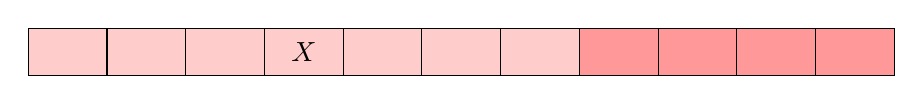
\begin{tikzpicture}[x=1cm, y=0cm, node distance=0cm,outer sep = 0pt]
\tikzstyle{gene}=[rectangle,draw,minimum width=1cm,minimum height=0.6cm]
\tikzstyle{aa}=[gene,fill=red!20]
\tikzstyle{al}=[gene,fill=red!40]

\node[aa] at (1,0) {};
\node[aa] at (2,0) {};
\node[aa] at (3,0) {};
\node[aa] at (4,0) {$X$};
\node[aa] at (5,0) {};
\node[aa] at (6,0) {};
\node[aa] at (7,0) {};
\node[al] at (8,0) {};
\node[al] at (9,0) {};
\node[al] at (10,0) {};
\node[al] at (11,0) {};

\end{tikzpicture}
\end{center}


\begin{center}
Απόγονος$A$:
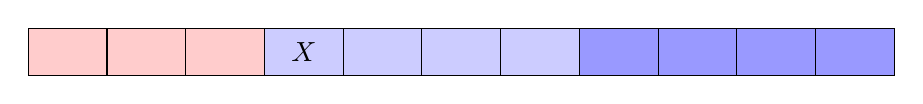
\begin{tikzpicture}[x=1cm, y=0cm, node distance=0cm,outer sep = 0pt]
\tikzstyle{gene}=[rectangle,draw,minimum width=1cm,minimum height=0.6cm]
\tikzstyle{aa}=[gene,fill=red!20]
\tikzstyle{al}=[gene,fill=red!40]
\tikzstyle{ba}=[gene,fill=blue!20]
\tikzstyle{bl}=[gene,fill=blue!40]

\node[aa] at (1,0) {};
\node[aa] at (2,0) {};
\node[aa] at (3,0) {};
\node[ba] at (4,0) {$X$};
\node[ba] at (5,0) {};
\node[ba] at (6,0) {};
\node[ba] at (7,0) {};
\node[bl] at (8,0) {};
\node[bl] at (9,0) {};
\node[bl] at (10,0) {};
\node[bl] at (11,0) {};

\end{tikzpicture}
\end{center}


\begin{center}
Γονέας$B$:\hspace*{5mm}
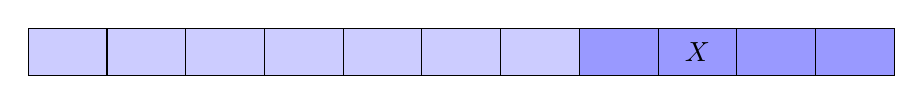
\begin{tikzpicture}[x=1cm, y=0cm, node distance=0cm, outer sep = 0pt]
\tikzstyle{gene}=[rectangle,draw,minimum width=1cm,minimum height=0.6cm]
\tikzstyle{ba}=[gene,fill=blue!20]
\tikzstyle{bl}=[gene,fill=blue!40]

\node[ba] at (1,0) {};
\node[ba] at (2,0) {};
\node[ba] at (3,0) {};
\node[ba] at (4,0) {};
\node[ba] at (5,0) {};
\node[ba] at (6,0) {};
\node[ba] at (7,0) {};
\node[bl] at (8,0) {};
\node[bl] at (9,0) {$X$};
\node[bl] at (10,0) {};
\node[bl] at (11,0) {};

\end{tikzpicture}
\end{center}





\begin{center}
Απόγονος$B$:
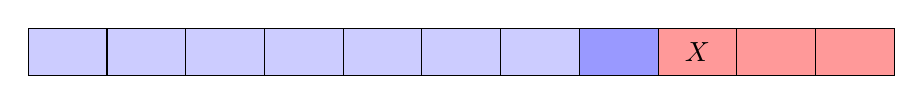
\begin{tikzpicture}[x=1cm, y=0cm, node distance=0cm, outer sep = 0pt]
\tikzstyle{gene}=[rectangle,draw,minimum width=1cm,minimum height=0.6cm]
\tikzstyle{ba}=[gene,fill=blue!20]
\tikzstyle{bl}=[gene,fill=blue!40]
\tikzstyle{aa}=[gene,fill=red!20]
\tikzstyle{al}=[gene,fill=red!40]

\node[ba] at (1,0) {};
\node[ba] at (2,0) {};
\node[ba] at (3,0) {};
\node[ba] at (4,0) {};
\node[ba] at (5,0) {};
\node[ba] at (6,0) {};
\node[ba] at (7,0) {};
\node[bl] at (8,0) {};
\node[al] at (9,0) {$X$};
\node[al] at (10,0) {};
\node[al] at (11,0) {};

\end{tikzpicture}
\end{center}
  \caption{Διαδικασία Διασταύρωσης στον GMl-ASLCS$_{\:0}$.}
  \label{fig:singlePointCrossoverOffsprings}
\end{figure}

Ο τελεστής της διασταύρωσης εφαρμόζεται με πιθανότητα $\chi = 0.8$. Σε περίπτωση απόφασης μη διασταύρωσης, οι απόγονοι βγαίνουν αλώβητοι από τη διαδικασία της διασταύρωσης, ως κλώνοι των γονέων τους. Σε κάθε περίπτωση, στη συνέχεια, και κατά τα γνωστά, εφαρμόζεται ο τελεστής της \emph{ομοιόμορφης μετάλλαξης}, δηλαδή κάθε γνώρισμα και ετικέτα υπόκειται ξεχωριστά σε μετάλλαξη, με πιθανότητα $\mu = 0.04$. 


\subsubsection{Διαδικασία εισαγωγής απογόνων στον πληθυσμό}
Κάθε κανόνας που έχει δημιουργηθεί μέσω του Γενετικού Αλγορίθμου, προτού εισαχθεί στον πληθυσμό (συνάρτηση $insert$ στον Αλγ. \ref{alg:gmlaslcs0Update}), ελέγχεται για \emph{υπαγωγή} (subsumption) ως προς το σύνολο των κανόνων. Εάν υπάρχει κάποιος κανόνας $r$ με εμπειρία μεγαλύτερη από ένα κατώφλι $\theta_{sub}$, με καταλληλότητα μεγαλύτερη από ένα κατώφλι καταλληλότητας $\alpha_{0}$, το ίδιο γενικός ή γενικότερος από το νέο κανόνα (απόγονο) στο τμήμα συνθήκης και, ταυτόχρονα, το ίδιο ειδικός ή ειδικότερος στο τμήμα απόφασης, ο απόγονος δεν εισάγεται στον πληθυσμό, αλλά αφομοιώνεται από τον $r$, αυξάνοντας την πληθικότητα του τελευταίου κατά ένα. Σε αντίθετη περίπτωση, ο κανόνας-απόγονος εισάγεται απευθείας στον πληθυσμό ως αυτοτελής κανόνας, χωρίς κάποια περαιτέρω διαδικασία.

Στην περίπτωση της δημιουργίας κανόνων μέσω της λειτουργίας κάλυψης, οι απόγονοι παρακάμπτουν τη διαδικασία αφομοίωσης και εισάγονται αυτοτελώς στον πληθυσμό.


\subsubsection{Λειτουργία Διαγραφής}
Όπως και στα σχήματα αναπαραγωγής των UCS και AS-LCS, έτσι και εδώ, το σύστημα εξελίσσει ένα σύνολο από κανόνες του οποίου το άθροισμα των πληθικοτήτων παραμένει κάτω από ένα συγκεκριμένο όριο, εκ των προτέρων επιλεγμένο από τον χρήστη. Κάθε φορά που συμβαίνει ένα γενετικό γεγονός, σύμφωνα με τα παραπάνω, έχουμε ως αποτέλεσμα την αύξηση του συνολικού αριθμού των κανόνων (και των μικρο-κανόνων) κατά δύο (δύο απόγονοι), είτε το αποτέλεσμα του γενετικού συμβάντος αφομοιωθεί, είτε εισαχθεί ακέραιο στον πληθυσμό. Στην περίπτωση που ο αριθμός των μικρο-κανόνων, πριν την εισαγωγή ενός απογόνου στον πληθυσμό είναι ίσος με το μέγιστο αριθμό μικρο-κανόνων που μπορεί να συγκρατήσει το σύστημα, ενεργοποιείται η λειτουργία της διαγραφής (γραμμές $20$ και $21$ στον Αλγ. \ref{alg:gmlaslcs0Update}), η οποία επιλέγει κανόνες προς διαγραφή χρησιμοποιώντας επιλογή ρουλέτας. Σε κάθε κανόνα ανατίθεται μία πιθανότητα διαγραφής ίση με 


\begin{equation}
\label{eq:deletionRoulette}
P(i) = \frac{num(i) \cdot d(i)}{\sum\limits_{j=1}^n \big(num(j) \cdot d(j)\big)}
\end{equation}
\\
όπου $i$ ένας τυχαίος κανόνας, $n$ ο συνολικός αριθμός κανόνων του πληθυσμού και

\begin{equation}
\label{eq:deletion_original}
d(i) = \left\{
\begin{array}{ c l }
0, & coverage(i) = 0$ ή $(coverage(i) = 1$ και $experience(i) = 1)
\\
\\
\displaystyle\frac{1}{100 \cdot fitness(i)}, & experience(i) < \theta_{del}
\\
\\
\displaystyle e^{\displaystyle cs(i)-1} ,& $αλλού$
\end{array}
\right.
\end{equation}
\\
όπου $coverage(i)$ το ποσοστό δειγμάτων του συνόλου εκπαίδευσης που καλύπτει ο κανόνας $i$, $experience(i)$ η εμπειρία του και $fitness(i)$ η τιμή καταλληλότητάς του (χωρίς έκπτωση βασισμένη στην εμπειρία, όπως αναφέρεται στη γρ. $7$ του Αλγ. \ref{alg:gmlaslcs0UpdateFitness}).



\subsection{Λειτουργία Κάλυψης}
\label{subsec:multiLabelCover}
Η λειτουργία της κάλυψης έχει σκοπό την κατασκευή κανόνων με βάση το τρέχον δείγμα $s$, με το οποίο εκπαιδεύεται το σύστημα. Ενεργοποιείται για κάθε ετικέτα όταν δεν υπάρχει κανένας κανόνας που να καλύπτει το δείγμα $s$. Επιπλέον, ενεργοποιείται για τις ετικέτες για τις οποίες υπάρχουν κανόνες που καλύπτουν το δείγμα, αλλά η απόφασή τους δεν συνάδει με αυτή του δείγματος (κενό $[C_{l}]$). Στη μονοκατηγορική ταξινόμηση, ο τελεστής κάλυψης δημιουργεί έναν κανόνα γενικεύοντας τυχαία τα γνωρίσματα του $s$ και μεταφέροντας αυτούσια την κλάση του δείγματος ως απόφαση του κανόνα. Στην πολυκατηγορική ταξινόμηση, όμως, δεδομένης της αναπαράστασης με αδιαφορίες που επεκτείνεται και στο τμήμα απόφασης των κανόνων, υπάρχει η δυνατότητα γενίκευσης και με βάση το τμήμα ετικετών των δειγμάτων. Έτσι, ένα γνώρισμα γενικεύεται (απενεργοποιείται) με πιθανότητα $P_{\#A}$, ενώ μία ετικέτα μπορεί να απενεργοποιηθεί και αυτή, με πιθανότητα $P_{\#L}$. 

Στα περισσότερα πραγματικά προβλήματα, $P_{\#L} \ll P_{\#A}$, καθώς, δεν θα θέλαμε να ωθήσουμε το σύστημα σε μία κατεύθυνση όπου θα συγκρατούσε ένα πληθυσμό από γενικούς κανόνες στο τμήμα απόφασης, σε βάρος λίγων, ειδικών στο τμήμα απόφασής τους κανόνων. Αυτή η απαίτηση γίνεται κατανοητή και από τη σκοπιά της ψηφοφορίας, που περιγράφεται στην Παρ. \ref{subsec:multiLabelVoting}. Ανεξαρτήτως, όμως, των πιθανοτήτων γενίκευσης $P_{\#L}$ και $P_{\#A}$, ένας τρόπος για να οδηγήσουμε το σύστημα στη δημιουργία κανόνων γενικών στο τμήμα συνθήκης και ειδικών στο τμήμα απόφασης είναι η “τιμωρία" των κανόνων για κάθε αδιαφορία στο τμήμα απόφασης τους. 


\subsection{Αφαίρεση των κανόνων μηδενικής κάλυψης}
Ενδιαφέρον παρουσιάζουν οι γραμμές $24$ και $25$ του Αλγ. \ref{alg:gmlaslcs0Update}. Αφού ενημερωθούν οι παράμετροι των κανόνων που συμμετέχουν στο Match Set και τα διάφορα Correct Sets, φροντίζουμε να απομακρύνουμε από τον πληθυσμό τους κανόνες μηδενικής κάλυψης, δηλαδή εκείνους τους κανόνες στους οποίους έχουν παρουσιαστεί όλα τα δείγματα του συνόλου δεδομένων, αλλά δεν έχουν συμμετάσχει σε κανένα σχηματιζόμενο Match Set. Κάθε τέτοιος κανόνας χαρακτηρίζεται από την απουσία νοήματος πάνω στο πρόβλημα, καθώς δεν καλύπτει ούτε ένα δείγμα του συνόλου εκπαίδευσης. Τέτοιοι κανόνες παράγονται μόνο από το Γενετικό Αλγόριθμο, και όχι από το τμήμα Κάλυψης\footnote{Η παραγωγή κανόνων μηδενικής κάλυψης, στην ουσία οφείλεται στη μη πληρότητα των πραγματικών συνόλων δεδομένων, δηλαδή στην απουσία δειγμάτων που να καθιστούν το σύνολο δεδομένων πλήρες ως προς όλους τους συνδυασμούς των τιμών των γνωρισμάτων.}. 

Ένα μέρος των κανόνων μηδενικής κάλυψης θα διαγραφεί από τον πληθυσμό, μετά το πέρας του κύκλου ενημέρωσης και παραγωγής κανόνων, με πιθανότητα αντιστρόφως ανάλογη του μεγέθους του συνόλου εκπαίδευσης $D$. Οι κανόνες που θα διαγραφούν έχουν δύο ιδιότητες: α) κάθε κανόνας πρέπει να έχει κληθεί να συμμετάσχει τουλάχιστον μία φορά σε Match Set για \emph{κάθε} δείγμα του $D$ και β) ο χρόνος παραγωγής του κανόνα θα πρέπει να είναι τέτοιος ώστε ο αριθμός κλήσεων συμμετοχής του σε $[M]$, δηλαδή ο αριθμός δειγμάτων που έχουν παρουσιαστεί στον κανόνα, να είναι ακέραιο πολλαπλάσιο του αριθμού δειγμάτων του $D$.


\subsection{Αρχικοποίηση Παραμέτρων Κανόνων}
Οι κανόνες που παράγονται μέσω της λειτουργίας κάλυψης έχουν αρχικές παραμέτρους $(tp, msa, cs, fitness) \equiv (0,0,20,0.5)$, ενώ αυτοί που δημιουργούνται μέσω του γενετικού αλγορίθμου $(0,0,(parentA.cs+parentB.cs)/2, 0.5)$. Δηλαδή, ένας κανόνας που παράγεται μέσω του Γενετικού Αλγορίθμου κληρονομεί ως $cs$ το μέσο όρο των $cs$ των δύο γονέων του, $parentA$ και $parentB$. Η αρχική καταλληλότητα ασκεί (περιορισμένα) επιρροή μόνο στη λειτουργία της διαγραφής, μέχρι ένας κανόνας να συμμετάσχει σε κάποιο Match Set. 



\section{Συνιστώσα Επίδοσης}
\label{sec:multiLabelInference}
Η συνιστώσα επίδοσης, όπως αναφέραμε στην Παρ. \ref{subsec:multiLabelInference}, είναι υπεύθυνη για την κατηγοριοποίηση ενός αγνώστου δείγματος με βάση το σύνολο των κανόνων που έχει εξελίξει το ΜαΣΤ. Σε αυτή την παράγραφο αναλύουμε τη μέθοδο ψηφοφορίας των κανόνων που χρησιμοποιεί ο GMl-ASLCS$_{\:0}$ και τη διαδικασία ρύθμισης του κατωφλίου με τη μέθοδο PCut.

\subsection{Μέθοδος Ψηφοφορίας}
\label{subsec:multiLabelVoting}
Η διαδικασία ξεκινάει με την είσοδο ενός άγνωστου δείγματος $s$ στο σύστημα. Από το σύνολο των κανόνων του πληθυσμού, συγκεντρώνονται στο $[M]$, κατά τα γνωστά, οι κανόνες που καλύπτουν το $s$. Στη συνέχεια, σχηματίζεται ο μονοδιάστατος, κενός πίνακας ψηφοφορίας $A$, μεγέθους $\abs{L}$, όπου $\abs{L}$ ο αριθμός των ετικετών των δειγμάτων. Ακολούθως, κάθε κανόνας του $[M]$ καλείται να ψηφίσει για την κάθε ετικέτα ξεχωριστά, με τον εξής τρόπο: οι κανόνες που συνηγορούν στην κατηγοριοποίηση στην ετικέτα $l \in L$ ψηφίζουν με θετικό πρόσημο, με την ποσότητα $num \times fitness$. Οι κανόνες που αρνούνται την κατάταξη του δείγματος στην $l$ ψηφίζουν με την ανωτέρω ποσότητα, αλλά με αρνητικό πρόσημο και αυτοί που αδιαφορούν για την $l$ δεν συμβάλλουν καθόλου στην ψηφοφορία. 

Για να γίνει περισσότερο κατανοητή η συνέχεια της διαδικασίας, ας υποθέσουμε ένα δείγμα $s_{0}: x \Rightarrow 100$, $[M] = \{r_{0}, r_{1}\}
$,  $r_{0}: x_{0} \Rightarrow 110$ και $r_{1}: x_{1} \Rightarrow 1\#1$, με τις εξής παραμέτρους: $num_{0} = 10$, $num_{1} = 20$, $fitness_{0} = 1$, $fitness_{1} = 0.8$, για ένα πρόβλημα τριών ετικετών ($\abs{L}=3$). Τότε, ο πίνακας $A_{0}$ που σχηματίζεται μετά την ψηφοφορία για το δείγμα $s_{0}$ είναι ο εξής:


\begin{center}
\begin{tikzpicture}
\node[align=center,draw,shape=rectangle split,rectangle split horizontal,rectangle split parts=3, text width=3cm] (A) at (0,0) 
{$1 \cdot 10 + 0.8 \cdot 20$
\nodepart{two}$-1 \cdot 10$
\nodepart{three}$1 \cdot 10 - 0.8 \cdot 20$};
\end{tikzpicture}
\end{center}

δηλαδή 

\begin{center}
\begin{tikzpicture}
\node[align=center,draw,shape=rectangle split,rectangle split horizontal,rectangle split parts=3, text width=2cm] (A) at (0,0) 
{$26$
\nodepart{two}$-10$
\nodepart{three}$-6$};
\end{tikzpicture}
\end{center}

Στη συνέχεια, η απόλυτη τιμή της μικρότερης αρνητικής ποσότητας ανάμεσα στις ετικέτες προστίθεται σε όλα τα αποτελέσματα και γίνεται κανονικοποίηση, χρησιμοποιώντας το άθροισμα των ψήφων:


\begin{center}
\begin{tikzpicture}
\node[align=center,draw,shape=rectangle split,rectangle split horizontal,rectangle split parts=3, text width=2cm] (A) at (0,0) 
{$36$
\nodepart{two}$0$
\nodepart{three}$4$};
\end{tikzpicture}
\end{center}

και 

\begin{center}
\begin{tikzpicture}
\node[align=center,draw,shape=rectangle split,rectangle split horizontal,rectangle split parts=3, text width=2cm] (A) at (0,0) 
{$36/40$
\nodepart{two}$0$
\nodepart{three}$4/40$};
\end{tikzpicture}
\end{center}

καταλήγοντας στον πίνακα

\begin{center}
\begin{tikzpicture}
\node[align=center,draw,shape=rectangle split,rectangle split horizontal,rectangle split parts=3, text width=2cm] (A) at (0,0) 
{$0.9$
\nodepart{two}$0$
\nodepart{three}$0.1$};
\end{tikzpicture}
\end{center}

Για κάθε δείγμα του συνόλου ελέγχου, λοιπόν, γίνεται η παραπάνω διαδικασία, με αποτέλεσμα ένα διδιάστατο πίνακα, με τόσες γραμμές όσα είναι τα δείγματα του συνόλου ελέγχου και τόσες στήλες όσες είναι ο αριθμός των ετικετών. Ακολούθως, υπολογίζεται το κατώφλι, το οποίο χαράσσει με οριζόντιο τρόπο την τελική κατηγοριοποίηση: δείγματα που στον πίνακα ψηφοφορίας τους $A$ έχουν τιμές μεγαλύτερες από το κατώφλι στις θέσεις που αντιστοιχούν σε συγκεκριμένες ετικέτες, κατηγοριοποιούνται στις ετικέτες αυτές. Προφανώς, δείγματα που στον πίνακα $A$ τους έχουν τιμές μικρότερες από το κατώφλι στις θέσεις που αντιστοιχούν σε συγκεκριμένες ετικέτες, δεν κατηγοριοποιούνται σε αυτές.

Σε συνέχεια του παραδείγματος, έστω ότι το υπολογιζόμενο κατώφλι παίρνει τιμή $t = 0.2$, τότε το δείγμα κατηγοριοποιείται πλήρως ορθά, καθώς το σύστημα αποφαίνεται πως πρέπει να κατηγοριοποιηθεί μόνο στην πρώτη ετικέτα και όχι στις άλλες δύο, όπως είναι και η πραγματική κατηγοριοποίηση για το $s_{0}$.


Στην παραπάνω διαδικασία, η καταλληλότητα $fitness$ είναι μεν συνάρτηση της ακρίβειας του κάθε κανόνα, μπορεί, όμως, να μην ταυτίζεται με το μέγεθος που χρησιμοποιήθηκε για την εξελικτική διαδικασία (Εξ. \ref{eq:fitnessDiscount}). Συγκεκριμένα, στο \cite{2000697} αναφέρεται πως διαφορετικά προβλήματα, απαιτούν διαφορετικές προσεγγίσεις για τη βελτιστοποίηση της κατηγοριοποίησης, όσον αφορά στην παράμετρο $\nu$. Η παράμετρος $\nu$ χρησιμοποιείται για να δώσει μεγαλύτερη βαρύτητα στην ακρίβεια των κανόνων, ώστε να τους καταστήσει περισσότερο διαχωρίσιμους στην επιλογή τους από τις λειτουργίες του συστήματος, στρέφοντας την εξελικτική διαδικασία προς την ανακάλυψη κανόνων ακριβέστερων από τους προκατόχους τους. Στον GMl-ASLCS$_{\:0}$, η παράμετρος $\nu$ στη διαδικασία της ψηφοφορίας λαμβάνεται ίση με ένα, δηλαδή η ψηφοφορία, στην ουσία, γίνεται βάσει της \emph{ακρίβειας} των κανόνων και όχι της καταλληλότητάς τους. Επιπλέον, δεν εφαρμόζεται κάποιου είδους έκπτωση βασισμένη στην εμπειρία, αλλά χρησιμοποιείται η πραγματική τιμή της ακρίβειας των κανόνων.


Από τη διαδικασία της ψηφοφορίας εξάγουμε και μία εικόνα για τη βαρύτητα που έχει η εξέλιξη κανόνων με αδιαφορίες στο τμήμα απόφασής τους, όσον αφορά στην ικανότητα ορθής κατηγοριοποίησης από ένα ΜαΣΤ. Εάν για ένα δείγμα ενεργοποιείται ένα σύνολο κανόνων με μεγάλο περιεχόμενο αδιαφοριών στις ετικέτες, οι μη μηδενικές ψήφοι μειώνονται δραστικά, επιτρέποντας έτσι σε λίγους κανόνες να καθορίσουν στην ουσία, πιο άμεσα, την κατηγοριοποίηση των αγνώστων δειγμάτων και κάνοντας, επιπρόσθετα, τη διαδικασία εύρεσης κατωφλίου δυσχερέστερη. Αυτό το φαινόμενο ενισχύεται σε προβλήματα χαμηλής κατηγορικής πληθικότητας (σε προβλήματα δηλαδή όπου ενεργοποιείται ένας μικρός αριθμός ετικετών για κάθε δείγμα), καθώς η ελάχιστη αρνητική τιμή που αφαιρείται από όλα τα αποτελέσματα της ψηφοφορίας προστίθεται και στις ψήφους των ετικετών για τις οποίες δεν υπάρχει ουσιαστική ψηφοφορία (των ετικετών, δηλαδή, για τις οποίες υπάρχουν ελάχιστες μη μηδενικές ψήφοι). Τελικά, το δείγμα κατατάσσεται σε ένα σύνολο ετικετών που περιλαμβάνει ορθά τις λίγες ετικέτες στις οποίες ανήκει πραγματικά και, με μεγάλη πιθανότητα, λανθασμένα τις ετικέτες για τις οποίες υπήρξε μεγάλη αποχή στην ψηφοφορία.


\subsection{Μέθοδος ρύθμισης κατωφλίου PCut}
\label{subsec:pcutCalibration}
Όπως αναφέραμε και στην Παρ. \ref{subsec:multiLabelInference}, η μέθοδος PCut, η οποία παρουσιάζεται σε μορφή ψευδοκώδικα στον Αλγ. \ref {alg:pcut}, προσπαθεί να επιλέξει το σωστό αριθμό ετικετών κατά μέσο όρο για ένα σύνολο δεδομένων $G$. Ο αλγόριθμος εκτελείται επαναληπτικά για \emph{iterations} βήματα, και προσεγγίζει σταδιακά την αναζητούμενη τιμή κατωφλίου (παράμετρος $center$) με ολοένα μειούμενο βήμα \emph{step}, αξιοποιώντας την κυρτότητα της συνάρτησης

\begin{equation} 
err(th,LC) =\left| LC(D) - \left(\frac{1}{|G|}\sum_{i=1}^{|G|}\left|f_{th}(\bar{w_i})\right|\right)\right| 
\end{equation}  
\\
όπου $LC$ είναι η κατηγορική πληθικότητα του συνόλου εκπαίδευσης $D$ και $G$ το σύνολο δεδομένων με βάση το οποίο γίνεται η ρύθμιση του κατωφλίου. 


\begin{algorithm} 
 \caption{Μέθοδος ρύθμισης κατωφλίου \textsc{Pcut}}
\label{alg:pcut}
 \begin{algorithmic}[1]
  \STATE \textbf{\textsc{Pcut}}($center$, $step$, $iterations$, $LC$)
  \IF {$iterations = 0$}
    \RETURN
  \ENDIF
  \STATE $fleft \gets center-step/2$
  \STATE $cleft \gets center-step/4$
  \STATE $fright \gets center+step/2$
  \STATE $cright \gets center+step/4$
  \STATE $next \gets err(fleft,LC) $
  \STATE $minError \gets err(fleft,LC) $
  \FOR {$point \in  \{cleft, center, cright, fright\}$}
      \IF{$minError > err(point,LC)$}
	\STATE $next \gets point$
	\STATE $minError \gets err(point,LC)$
      \ENDIF
  \ENDFOR
  \STATE $\textbf{\textsc{Pcut}}(next,step/2,iterations-1,LC)$
 \end{algorithmic}
\end{algorithm}


Κλείνοντας, αξίζει να σημειώσουμε πως, στην περίπτωσή μας, τα σύνολα $D$ και $G$ ταυτίζονται πάντα, καθώς η χρήση του συνόλου ελέγχου στη θέση του $G$ υπονοεί εκ των προτέρων γνώση της δομής των ετικετών σε μη επισημασμένα δείγματα και οδηγεί σε υπερβολικά επιεικείς αξιολογήσεις.

 
